\documentclass[tikz, border=15pt]{standalone}
\usepackage{amsmath}
\usepackage{amsfonts}
\usetikzlibrary{calc, arrows.meta, positioning, decorations.pathreplacing}

\begin{document}

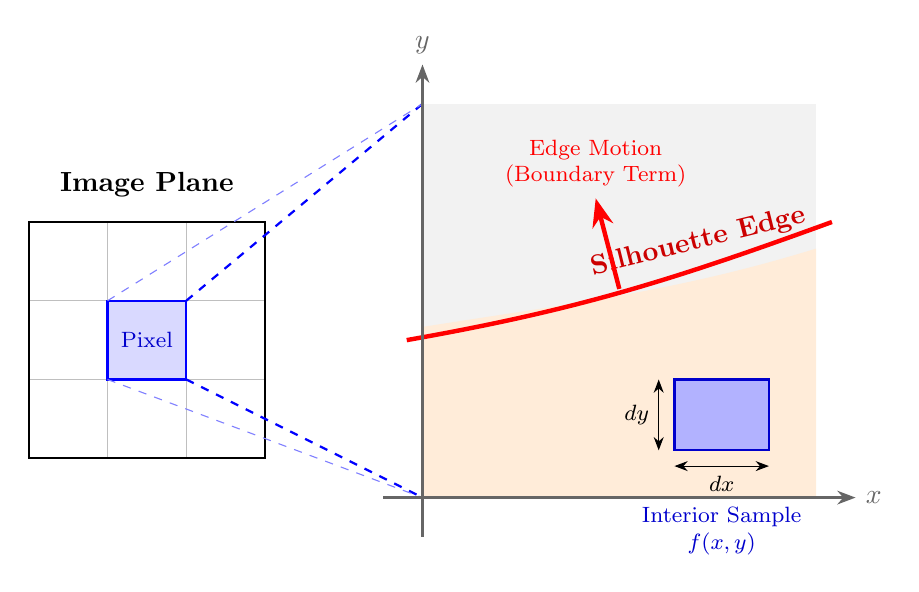
\begin{tikzpicture}[x=1cm, y=1cm, >=Stealth]

    % ==========================================
    % 1. LEFT SIDE: Full Image / Sensor Grid
    % ==========================================
    \node[anchor=south, font=\bfseries] at (1.5, 3.2) {Image Plane};
    
    % Draw the grid of pixels
    \draw[step=1cm, gray!50, thin] (0,0) grid (3,3);
    \draw[thick] (0,0) rectangle (3,3);

    % Highlight a single pixel being integrated
    \fill[blue!15] (1,1) rectangle (2,2);
    \draw[blue, thick] (1,1) rectangle (2,2);
    \node[font=\footnotesize, text=blue!80!black] at (1.5, 1.5) {Pixel};

    % ==========================================
    % 2. ZOOM EFFECT LINES
    % ==========================================
    \draw[dashed, blue, thick] (2,2) -- (5, 4.5);
    \draw[dashed, blue, thick] (2,1) -- (5, -0.5);
    \draw[dashed, blue!50, thin] (1,2) -- (5, 4.5);
    \draw[dashed, blue!50, thin] (1,1) -- (5, -0.5);

    % ==========================================
    % 3. RIGHT SIDE: Zoomed-in Pixel Space
    % ==========================================
    \begin{scope}[shift={(5,-0.5)}]
        
        % Base pixel background
        \fill[blue!2] (0,0) rectangle (5,5);

        % Foreground / Background split representing the visibility discontinuity
        \begin{scope}
            \clip (0,0) rectangle (5,5);
            % Background (e.g., scene behind object)
            \fill[gray!10] (0,0) rectangle (5,5);
            % Object (Foreground geometry occluding the background)
            \fill[orange!15] (-1,-1) -- (-1, 2) to[out=10, in=200] (6, 3.5) -- (6,-1) -- cycle;
        \end{scope}

        % % Draw the zoomed pixel boundary
        % \draw[blue, thick] (0,0) rectangle (5,5);
        % \node[anchor=south, font=\bfseries] at (2.5, 5.2) {Pixel Integral: $I = \iint k(x, y) L(x, y) \, dx \, dy$};

        % ==========================================
        % 4. THE SILHOUETTE EDGE (Dirac Delta Boundary)
        % ==========================================
        \draw[red, ultra thick] (-0.2, 2) to[out=10, in=200] (5.2, 3.5);
        \node[red!80!black, font=\bfseries, rotate=14] at (3.5, 3.25) {Silhouette Edge};

        % Arrow representing edge velocity / derivative (Li et al. explicit sampling)
        \draw[->, red, ultra thick] (2.5, 2.65) -- (2.2, 3.8) 
            node[above, font=\footnotesize, align=center] {Edge Motion\\(Boundary Term)};

        % ==========================================
        % 5. THE CONTINUOUS AREA ELEMENT (dx, dy)
        % ==========================================
        \begin{scope}[shift={(3.2, 0.6)}]
            % Area element box
            \fill[blue!30] (0,0) rectangle (1.2, 0.9);
            \draw[blue!80!black, thick] (0,0) rectangle (1.2, 0.9);

            % Center point of the sample
            % \fill[black] (0.6, 0.45) circle (1.5pt);
            % \node[anchor=south, font=\footnotesize] at (0.6, 0.45) {$(x,y)$};

            % Dimensions dx and dy with arrows
            \draw[<->] (0, -0.2) -- (1.2, -0.2) node[midway, below, font=\footnotesize] {$dx$};
            \draw[<->] (-0.2, 0) -- (-0.2, 0.9) node[midway, left, font=\footnotesize] {$dy$};

            % Callout mapping back to f(x,y)
            \node[anchor=north, font=\footnotesize, align=center, text=blue!80!black] 
                at (0.6, -0.6) {Interior Sample\\$f(x,y)$};
        \end{scope}

        % ==========================================
        % 6. LOCAL AXES
        % ==========================================
        \draw[->, thick, gray!80!black] (-0.5, 0) -- (5.5, 0) node[right] {$x$};
        \draw[->, thick, gray!80!black] (0, -0.5) -- (0, 5.5) node[above] {$y$};

    \end{scope}

\end{tikzpicture}

\end{document}